\documentclass{standalone}
\usepackage{tikz}
\usetikzlibrary{patterns, positioning}
\usepackage[sfdefault]{ClearSans} %% option 'sfdefault' activates Clear Sans as the default text font
\usepackage[T1]{fontenc}

\begin{document}
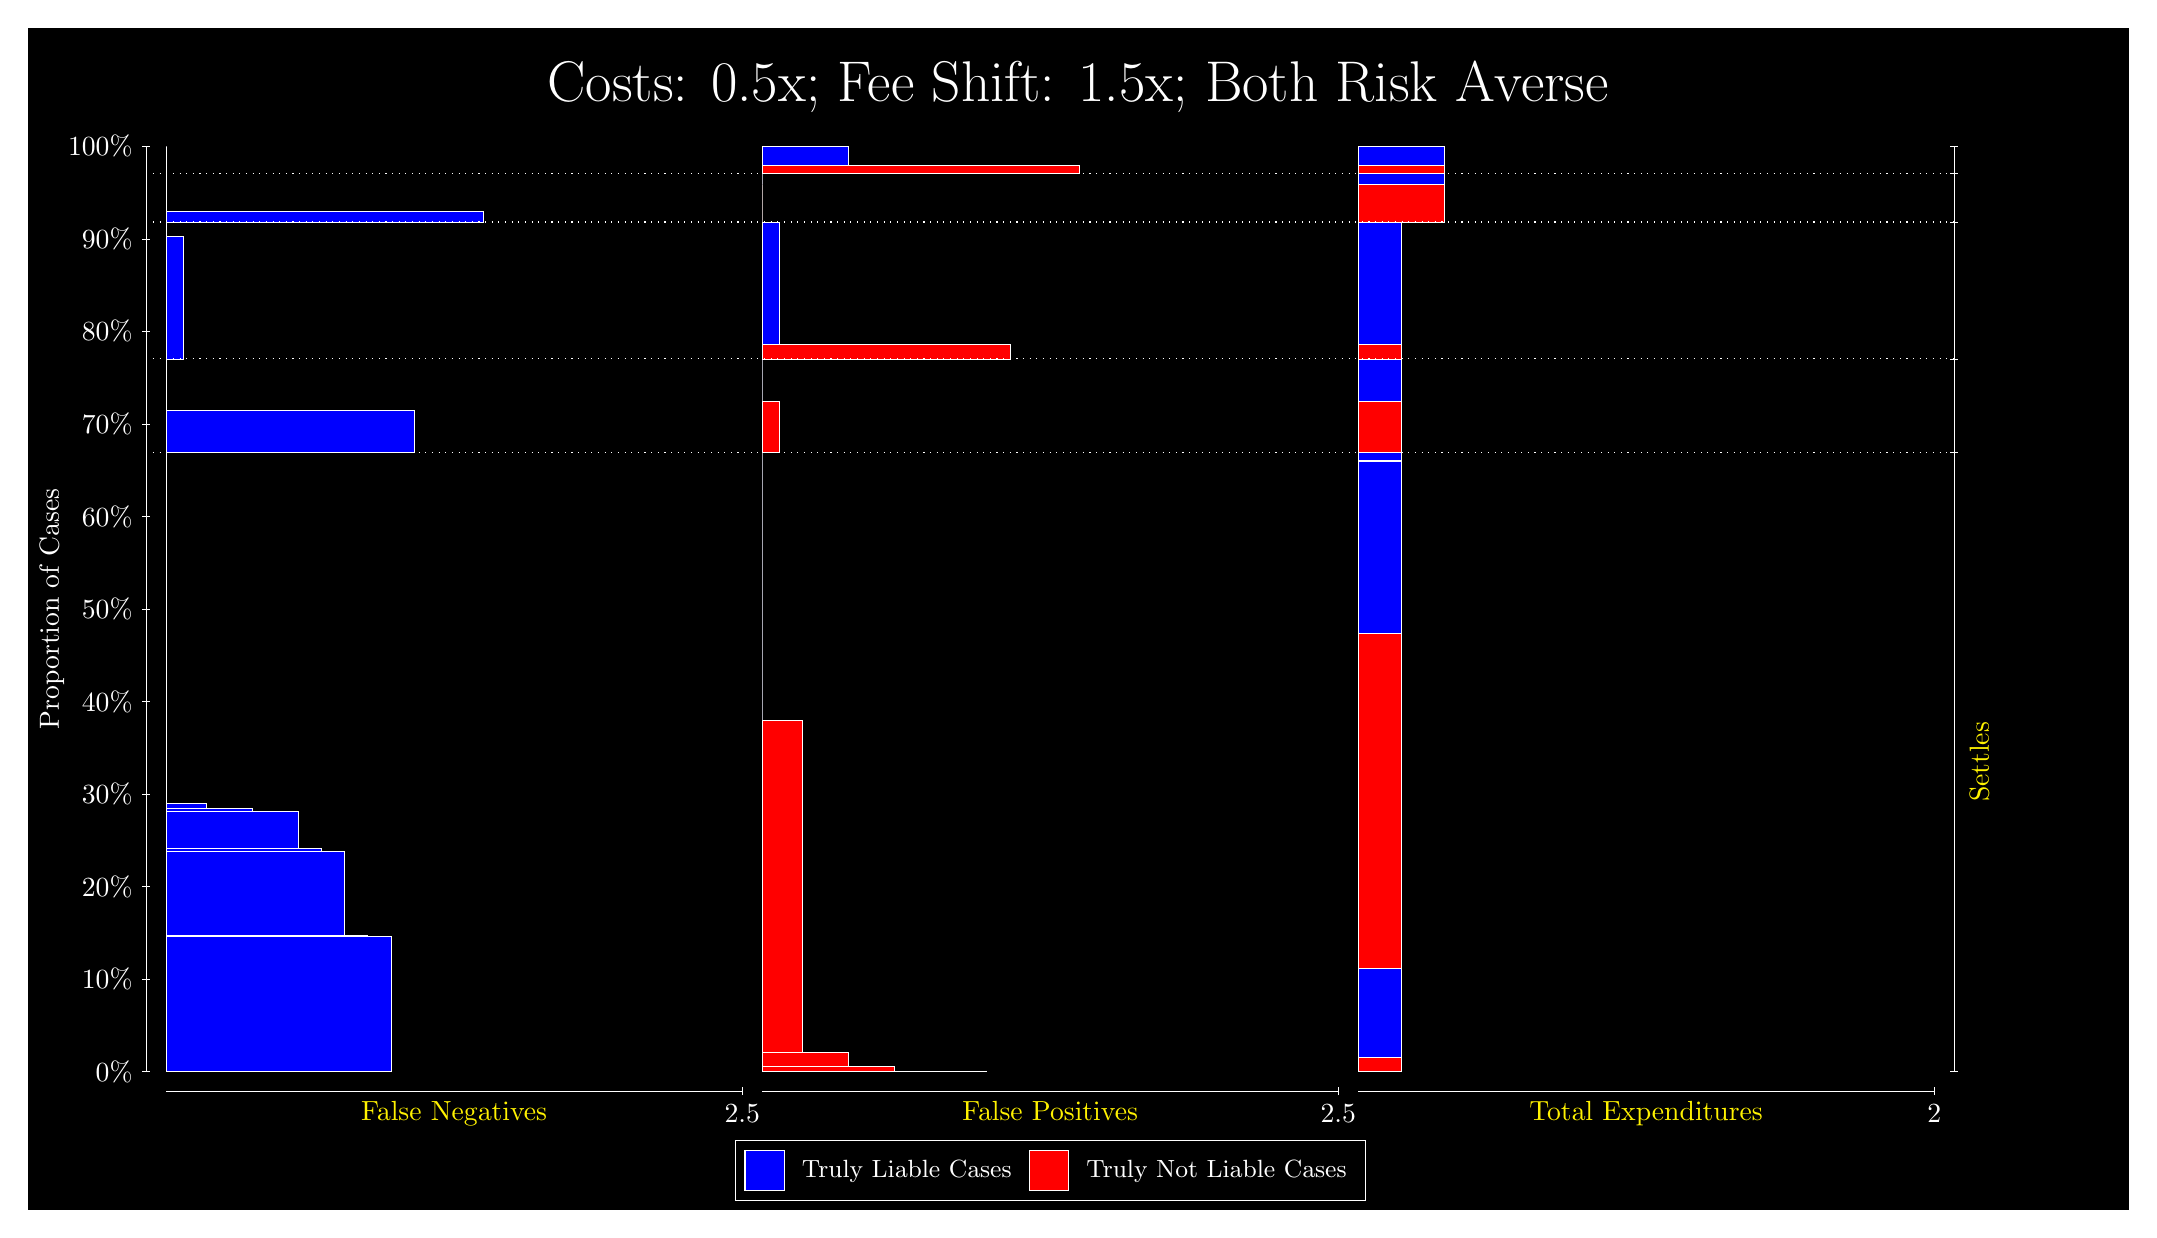
\begin{tikzpicture}
\draw[fill=black] (0,0) rectangle (26.667,15);
\draw[text=white] (0,13.5) rectangle (26.667,15) node[midway] {\huge Costs: 0.5x; Fee Shift: 1.5x; Both Risk Averse};
\draw[white, very thin] (1.5,1.75) -- (1.5,13.5);
\node[rotate=90, text=white, anchor=center] at (0.3, 7.625) {Proportion of Cases};
\draw[white, very thin] (1.45,1.75) -- (1.55,1.75);
\node[text=white, anchor=east] at (1.45, 1.75) {0\%};
\draw[white, very thin] (1.45,2.925) -- (1.55,2.925);
\node[text=white, anchor=east] at (1.45, 2.925) {10\%};
\draw[white, very thin] (1.45,4.1) -- (1.55,4.1);
\node[text=white, anchor=east] at (1.45, 4.1) {20\%};
\draw[white, very thin] (1.45,5.275) -- (1.55,5.275);
\node[text=white, anchor=east] at (1.45, 5.275) {30\%};
\draw[white, very thin] (1.45,6.45) -- (1.55,6.45);
\node[text=white, anchor=east] at (1.45, 6.45) {40\%};
\draw[white, very thin] (1.45,7.625) -- (1.55,7.625);
\node[text=white, anchor=east] at (1.45, 7.625) {50\%};
\draw[white, very thin] (1.45,8.8) -- (1.55,8.8);
\node[text=white, anchor=east] at (1.45, 8.8) {60\%};
\draw[white, very thin] (1.45,9.975) -- (1.55,9.975);
\node[text=white, anchor=east] at (1.45, 9.975) {70\%};
\draw[white, very thin] (1.45,11.15) -- (1.55,11.15);
\node[text=white, anchor=east] at (1.45, 11.15) {80\%};
\draw[white, very thin] (1.45,12.325) -- (1.55,12.325);
\node[text=white, anchor=east] at (1.45, 12.325) {90\%};
\draw[white, very thin] (1.45,13.5) -- (1.55,13.5);
\node[text=white, anchor=east] at (1.45, 13.5) {100\%};

\draw[white, very thin] (24.457,1.75) -- (24.457,13.5);
\draw[white, very thin] (24.407,1.75) -- (24.507,1.75);
\node[anchor=west] at (24.407, 1.75) {};
\draw[white, very thin] (24.407,9.6157) -- (24.507,9.6157);
\node[anchor=west] at (24.407, 9.6157) {};
\draw[white, very thin] (24.407,10.8) -- (24.507,10.8);
\node[anchor=west] at (24.407, 10.8) {};
\draw[white, very thin] (24.407,12.539) -- (24.507,12.539);
\node[anchor=west] at (24.407, 12.539) {};
\draw[white, very thin] (24.407,13.153) -- (24.507,13.153);
\node[anchor=west] at (24.407, 13.153) {};
\draw[white, very thin] (24.407,13.5) -- (24.507,13.5);
\node[anchor=west] at (24.407, 13.5) {};

\draw[white, very thin, fill=blue] (1.75,1.75) rectangle (4.6044,3.4667);
\draw[white, very thin, fill=blue] (1.75,3.4667) rectangle (4.3116,3.4857);
\draw[white, very thin, fill=blue] (1.75,3.4857) rectangle (4.0188,4.5455);
\draw[white, very thin, fill=blue] (1.75,4.5455) rectangle (3.7261,4.5873);
\draw[white, very thin, fill=blue] (1.75,4.5873) rectangle (3.4333,5.05);
\draw[white, very thin, fill=blue] (1.75,5.05) rectangle (3.1406,5.0604);
\draw[white, very thin, fill=blue] (1.75,5.0604) rectangle (2.8478,5.0896);
\draw[white, very thin, fill=blue] (1.75,5.0896) rectangle (2.5551,5.0961);
\draw[white, very thin, fill=blue] (1.75,5.0961) rectangle (2.2623,5.1587);
\draw[white, very thin, fill=red] (1.75,5.1587) rectangle (1.75,9.6157);
\draw[white, very thin, fill=blue] (1.75,9.6157) rectangle (4.8971,10.152);
\draw[white, very thin, fill=red] (1.75,10.152) rectangle (1.75,10.8);
\draw[white, very thin, fill=blue] (1.75,10.8) rectangle (1.9696,12.355);
\draw[white, very thin, fill=red] (1.75,12.355) rectangle (1.75,12.539);
\draw[white, very thin, fill=blue] (1.75,12.539) rectangle (5.7754,12.675);
\draw[white, very thin, fill=red] (1.75,12.675) rectangle (1.75,13.153);
\draw[white, very thin, fill=red] (1.75,13.153) rectangle (1.75,13.261);
\draw[white, very thin, fill=blue] (1.75,13.261) rectangle (1.75,13.5);
\draw[white, very thin, fill=red] (9.3189,1.75) rectangle (12.173,1.7536);
\draw[white, very thin, fill=red] (9.3189,1.7536) rectangle (11.88,1.754);
\draw[white, very thin, fill=red] (9.3189,1.754) rectangle (11.588,1.7557);
\draw[white, very thin, fill=red] (9.3189,1.7557) rectangle (11.295,1.7564);
\draw[white, very thin, fill=red] (9.3189,1.7564) rectangle (11.002,1.8127);
\draw[white, very thin, fill=red] (9.3189,1.8127) rectangle (10.709,1.8155);
\draw[white, very thin, fill=red] (9.3189,1.8155) rectangle (10.709,1.8169);
\draw[white, very thin, fill=red] (9.3189,1.8169) rectangle (10.417,1.9963);
\draw[white, very thin, fill=red] (9.3189,1.9963) rectangle (10.124,1.9976);
\draw[white, very thin, fill=red] (9.3189,1.9976) rectangle (9.8312,6.207);
\draw[white, very thin, fill=blue] (9.3189,6.207) rectangle (9.3189,9.6157);
\draw[white, very thin, fill=red] (9.3189,9.6157) rectangle (9.5384,10.264);
\draw[white, very thin, fill=blue] (9.3189,10.264) rectangle (9.3189,10.8);
\draw[white, very thin, fill=red] (9.3189,10.8) rectangle (12.466,10.985);
\draw[white, very thin, fill=blue] (9.3189,10.985) rectangle (9.5384,12.539);
\draw[white, very thin, fill=red] (9.3189,12.539) rectangle (9.3189,13.018);
\draw[white, very thin, fill=blue] (9.3189,13.018) rectangle (9.3189,13.153);
\draw[white, very thin, fill=red] (9.3189,13.153) rectangle (13.344,13.261);
\draw[white, very thin, fill=blue] (9.3189,13.261) rectangle (10.417,13.5);
\draw[white, very thin, fill=red] (16.888,1.75) rectangle (17.437,1.9349);
\draw[white, very thin, fill=blue] (16.888,1.9349) rectangle (17.437,3.0555);
\draw[white, very thin, fill=red] (16.888,3.0555) rectangle (17.437,7.3212);
\draw[white, very thin, fill=blue] (16.888,7.3212) rectangle (17.437,9.5006);
\draw[white, very thin, fill=red] (16.888,9.5006) rectangle (17.437,9.507);
\draw[white, very thin, fill=blue] (16.888,9.507) rectangle (17.437,9.6157);
\draw[white, very thin, fill=red] (16.888,9.6157) rectangle (17.437,10.264);
\draw[white, very thin, fill=blue] (16.888,10.264) rectangle (17.437,10.8);
\draw[white, very thin, fill=red] (16.888,10.8) rectangle (17.437,10.985);
\draw[white, very thin, fill=blue] (16.888,10.985) rectangle (17.437,12.539);
\draw[white, very thin, fill=red] (16.888,12.539) rectangle (17.986,13.018);
\draw[white, very thin, fill=blue] (16.888,13.018) rectangle (17.986,13.153);
\draw[white, very thin, fill=red] (16.888,13.153) rectangle (17.986,13.261);
\draw[white, very thin, fill=blue] (16.888,13.261) rectangle (17.986,13.5);
\draw[white, dotted] (1.5,9.6157) -- (24.457,9.6157);
\draw[white, dotted] (1.5,10.8) -- (24.457,10.8);
\draw[white, dotted] (1.5,12.539) -- (24.457,12.539);
\draw[white, dotted] (1.5,13.153) -- (24.457,13.153);
\draw[white, very thin] (1.75,1.5) -- (9.0689,1.5);
\node[text=yellow, anchor=north] at (5.4094, 1.5) {False Negatives};
\draw[white, very thin] (9.0689,1.45) -- (9.0689,1.55);
\node[text=white, anchor=north] at (9.0689, 1.45) {2.5};

\draw[white, very thin] (9.3189,1.5) -- (16.638,1.5);
\node[text=yellow, anchor=north] at (12.978, 1.5) {False Positives};
\draw[white, very thin] (16.638,1.45) -- (16.638,1.55);
\node[text=white, anchor=north] at (16.638, 1.45) {2.5};

\draw[white, very thin] (16.888,1.5) -- (24.207,1.5);
\node[text=yellow, anchor=north] at (20.547, 1.5) {Total Expenditures};
\draw[white, very thin] (24.207,1.45) -- (24.207,1.55);
\node[text=white, anchor=north] at (24.207, 1.45) {2};

\node[text=yellow, centered, rotate=90] at (24.777, 5.6829) {Settles};





\draw (12.978300999999998,1.5) node[draw=none] (baseCoordinate) {};
\begin{scope}[align=center]
        \matrix[scale=0.5, draw=white, below=0.5cm of baseCoordinate, nodes={draw}, column sep=0.1cm]{
            \node[rectangle, draw, minimum width=0.5cm, minimum height=0.5cm, fill=blue] {}; &
            \node[draw=none, font=\small, text=white] (B) {Truly Liable Cases}; &
            \node[rectangle, draw, minimum width=0.5cm, minimum height=0.5cm, fill=red] {}; &
            \node[draw=none, font=\small, text=white] (B) {Truly Not Liable Cases}; \\
            };
\end{scope}

\end{tikzpicture}
\end{document}